\section{Events}
	\subsubsection{Qualifying competitions}
		\begin{enumerate}
			\item Sochi.The first experience of team in the competition.At these competitions our squad for the first time felt the spirit of competition FCS and noble professionalism. Got work experience all day and all night. Began to make acquaintance among the teams simultaneously providing all possible pomosch.V plan and organization were all very nice. The most zapominayushimsya stlo familiarity with the American team Stuy fission 310, which is now supported by the connection.As a result we got a quota on the regional finals.
			\center{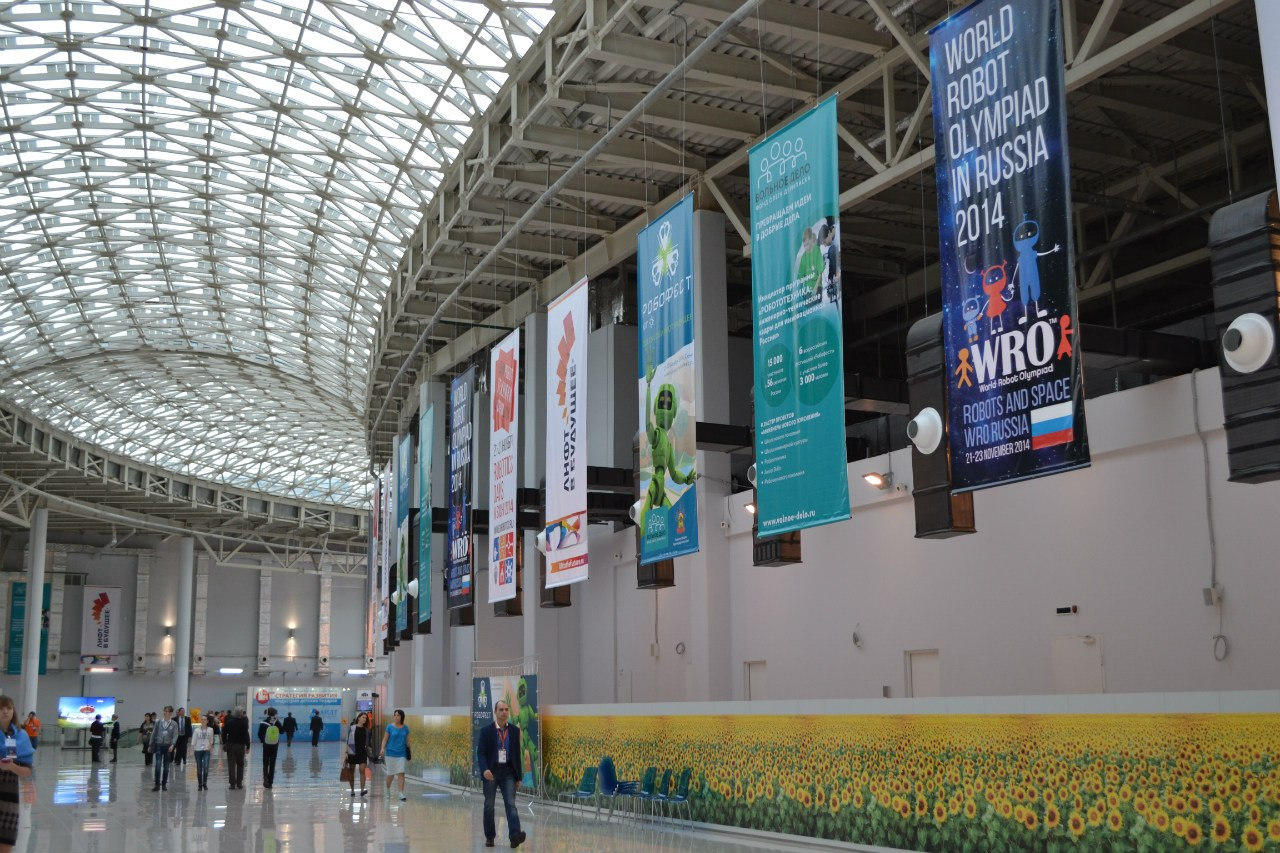
\includegraphics[scale=0.2]{days/Event/images/6}}\\
			\item Ryazan.In cutting our first priority train on a real field. These competitions were small enough and quiet. All teams abundantly communicated and shared ideas. There all feel comfortable.Team strongly helped to organize example - to assemble and disassemble the field. As a result Participants of the alliance winner. 
			\center{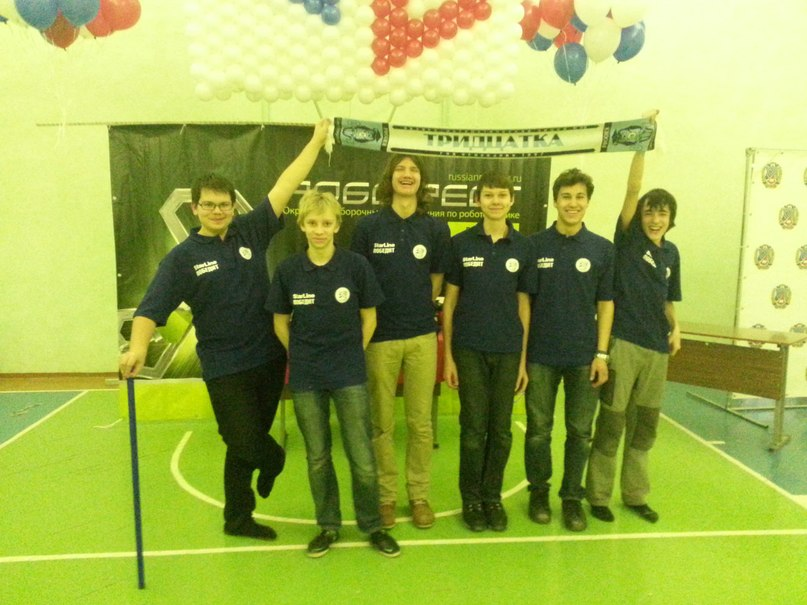
\includegraphics[scale=0.2]{days/Event/images/1}}\\	
			\item Permian.Dress rehearsal before the regional final. It was great organized event where we were able to practice all aspects of the competition. Including such important as the choice of Composes alliances finale.takzhe we strongly helped organizer with the technical part. As a result: the alliance of winners as well as first place in the general classification.
			\center{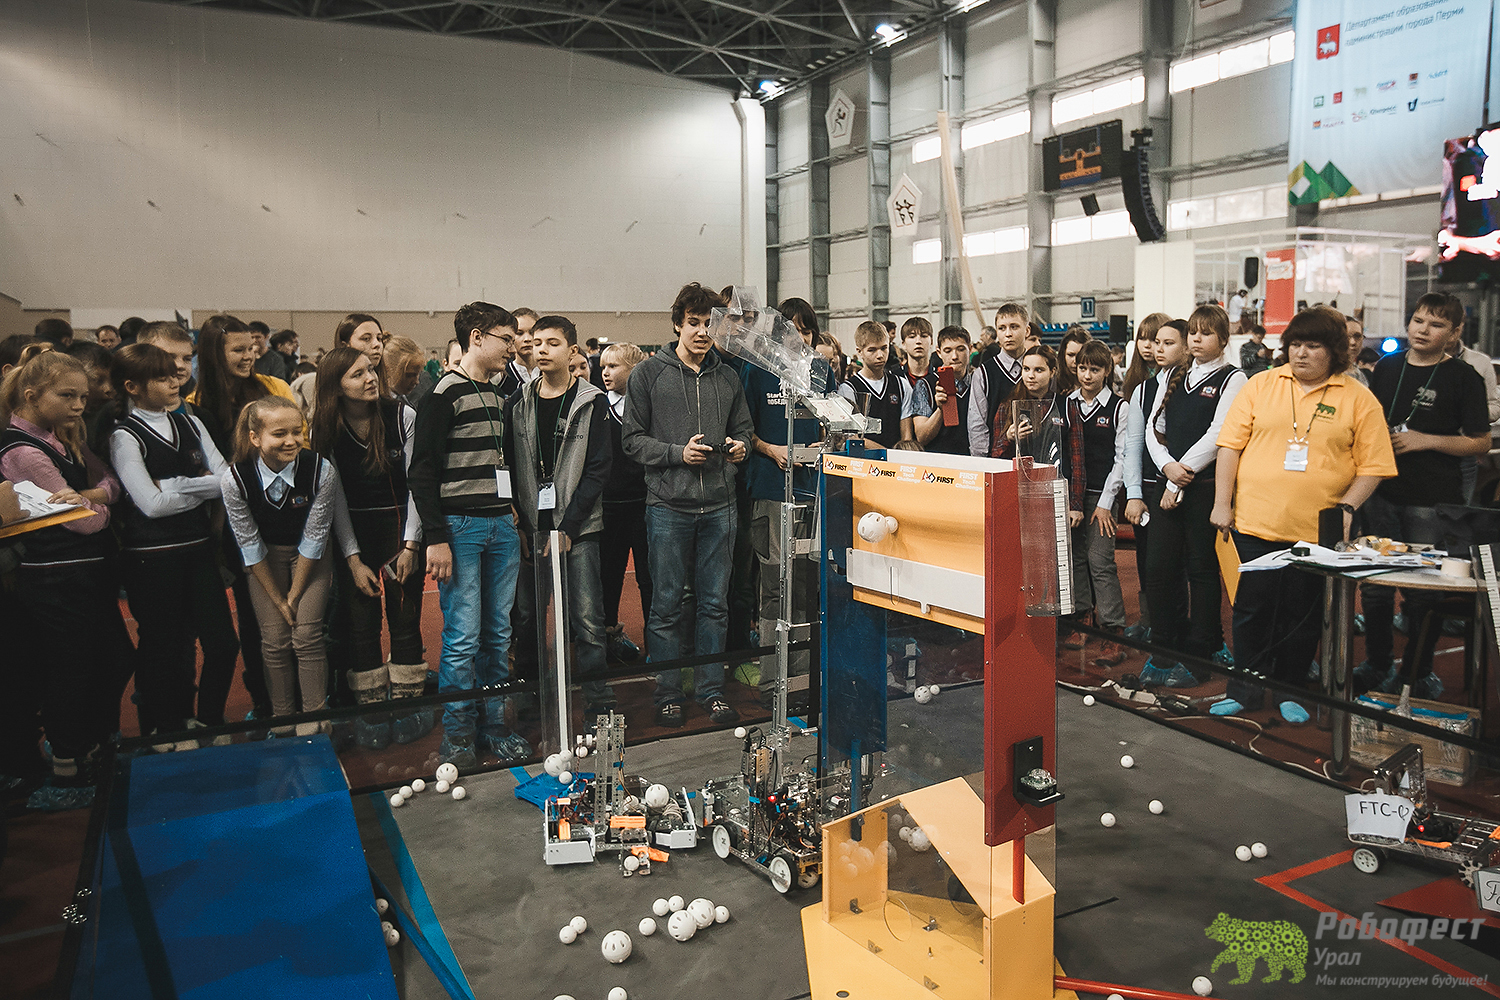
\includegraphics[scale=0.2]{days/Event/images/3}}\\
		\end{enumerate}  
	\subsubsection{Regional final}	
		The event to which the team was preparing for six months. Approaching the competition with fully finished. At competitions communicated with all the teams that were there, discussing strategy and offering their help. During the competition was conducted statistics on all the teams that helped in choosing allies in the final. Was also an action plan with any team. In the final, having received a quota on the choice of allies, were chosen team with the most stable results, and the rate was at komndnoe interaction of any pair of robots.As a result: the alliance of winners as well as first place in the general classification, and the quota to World Championship.
			\center{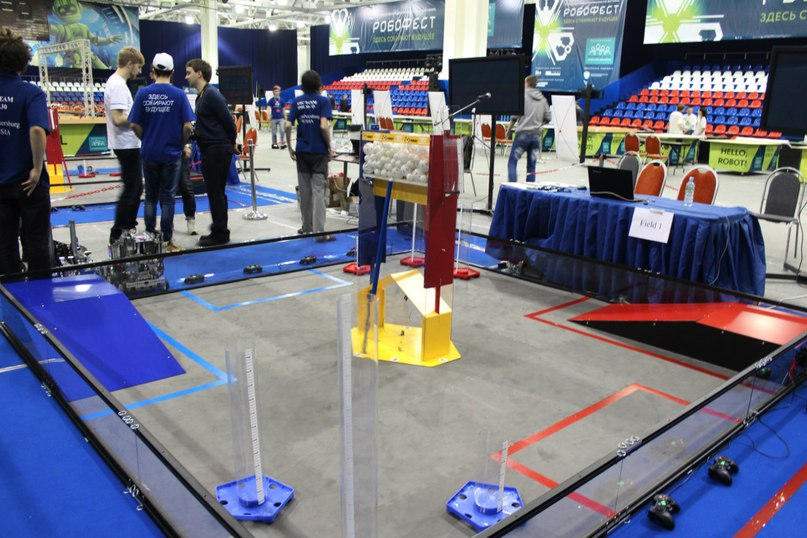
\includegraphics[scale=0.2]{days/Event/images/2}}\\
	\newpage			
	\subsubsection{CRDI RTC}
		Large Russian Institute of Robotics and Technical Cybernetics. The team was organized hike in instiut n can see the real processes develop detailed design for robotics. There saw several Projects summary at different stages of development - from drawing to finished models, as well as ready-made commercial products. From there we learned some ideas on how to organize. Internet adress http://www.rtc.ru.	\\
		\center{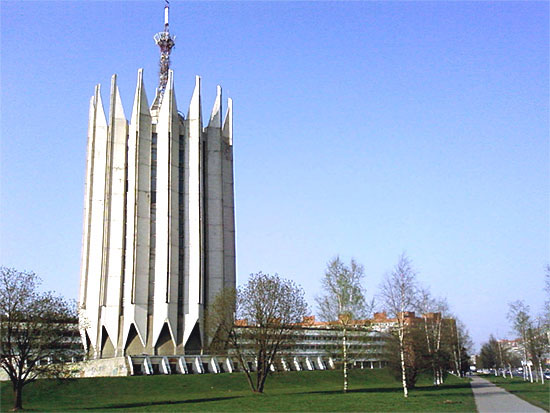
\includegraphics[scale=0.2]{days/Event/images/5}}\\
	\subsubsection{GeoScan}
		Russian company produces and sells unmanned aerial photography systems. There have clearly shown how the design office, as the allocation of responsibilities and tasks. How is the internal interaction. Also, we have shown the whole production line. Internet adress http://geoscan.aero/.	
		\center{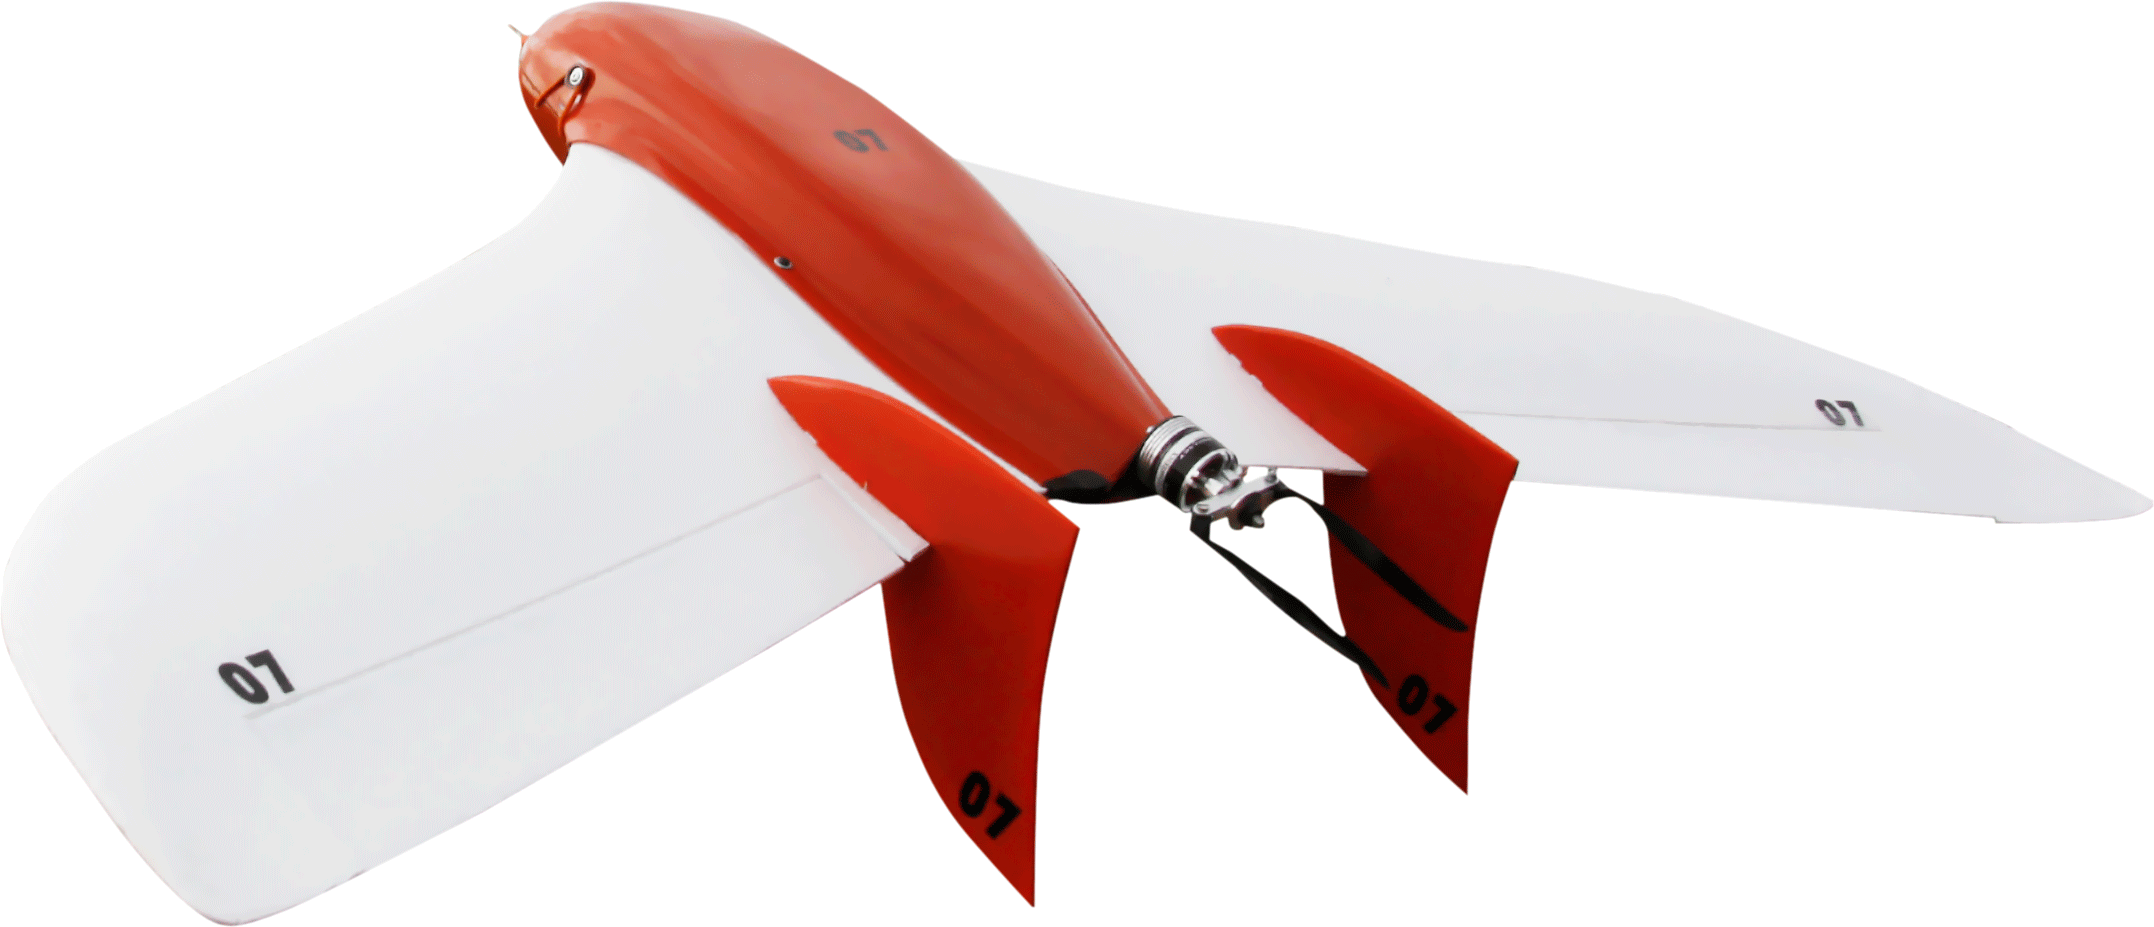
\includegraphics[scale=0.2]{days/Event/images/4}}\\
	\subsubsection{PML 30 landfill}	
		PML 30 landfill competitions are carried out by our organization. Their main sysl misrepresented that participant receives a rear and parts for its decision merely on the competition, compliance with the maximum being equal. We also demonstrated the FTC involving the participation.
		\center{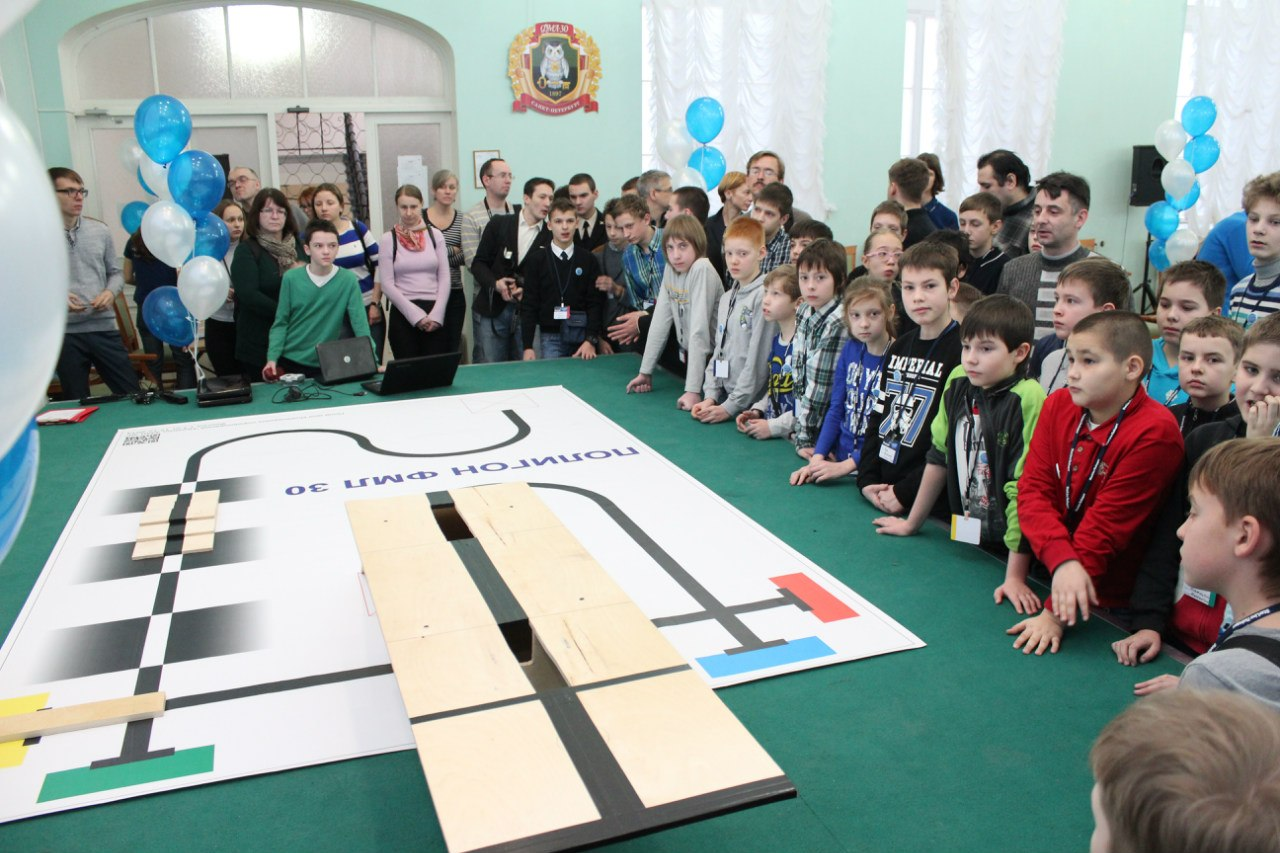
\includegraphics[scale=0.2]{days/Event/images/7}}\\
	\subsubsection{Summer camp on Robotics}
	In the camp in 2015, team members will conduct a robotics engineering course based on constructor TETRIX, attracting more people to the FTC.
		
		
		
		
		
		
		
		
		